\chapter{Wnioski}

App Inventor to sposób pomocy dla kogoś, kto nie miał styczności z programowaniem. Ogólnie rzecz biorąc istnieje kompromis pomiędzy programowaniem wizualnym, a programowaniem natywnym jeżeli chodzi o łatwość użycia, a ekspresywność i moc jaką daje znajomość Javy. Napisanie prostego \emph{Hello World} jest zazwyczaj łatwiejsze w środowiskach oferujących programowanie wizualne. W języku Java, który ma bardzo wiele zastosowań, aby stworzyć i zrozumieć prosty program wyświetlający napis \emph{Hello World} trzeba poznać wiele elementów Javy. Są to między innymi klasy, metody statyczne, pakiety, wywołania metod, różne strumienie do wyświetlenia danego tekstu, składnia języka. Jak widać jest to bardzo dużo elementów. 

Jednym z przykładów, który sprawia, że App Inventor jest nastawiony na przyszłych programistów jest numerowanie list od 1, zamiast od 0, co może wydawać się nieintuicyjne dla doświadczonych programistów. Głównie to co sprawia że programowanie wizualne jest nastawione na początkujących jest eliminacja możliwości popełnienia błędów składniowych, uniemożliwiając tym samym stworzenie niedziałających programów. 

Z drugiej strony stworzenie prostej funkcji wielomianowej: $4x^3+2x^2-5x+1$ może okazać się bardziej czasochłonne niż napisanie jej w Javie. 
Na poniższych rysunkach widać, że funkcja napisana w Javie może okazać się łatwiejsza w zrozumieniu.


\begin{figure}[H]
\centering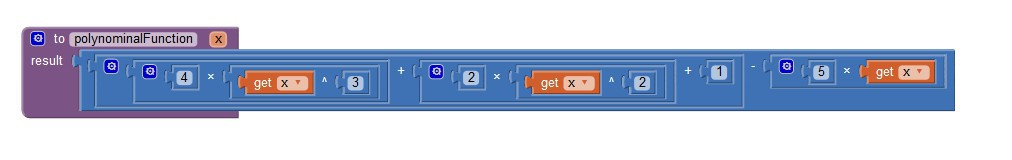
\includegraphics[width=15cm]{figures/polynominalFunction}
\caption{Bloki tworzące powyższą funkcję wielomianową}
\end{figure}

\begin{lstlisting}
int polynominalFunction(int x){
	return 4*pow(x,3)+2*pow(x,2)-5*x+1;
}
\end{lstlisting}


Podsumowująć niektóre gry, takie jak quizzy mogą być zaimplementowane za pomocą App Inventora, natomiast kiedy potrzebujemy płynnej animacji i stojącej za nią bardziej skomplikowanej logiki powinniśmy skorzystać z SDK, które oferuje nam Android. Języki blokowe wydają się być przeznaczone dla początkujących, więc projekty nie są tak zaawansowane, jak te, które są stworzone w języku natywnym. Korzystanie z bloków i przeciąganie ich jest nieporęczne dla złożonych programów.

Język wizualny jest przydatny, jeżeli programista ma na myśli proste projekty. Zawodzą one natomiast, jeżeli chodzi o zarządzanie na wielu poziomach abstrakcji i ziarnistości, jaką wymagają duże projekty. Mają one szansę odnieść sukces jako narzędzie, które będzie wyspecjalizowane w konkretnej domenie. System Android jest bardzo szybko rozrasta się i często pojawiają się nowe dostępne funkcjonalności. App Inventor jest narzędziem, który potrafi wykorzystać podstawowe, komponenty systemu Android, skupiając się na początkujących programistach. Jego celem nie są doświadczone osoby programujące od wielu lat, ponieważ, będą one chciały skorzystać z funkcji, które nie są dostępne.

Z drugiej strony można zauważyć, że programowanie wizualne jest coraz bardziej popularne. Główne środowiska programistyczne używane przez programistów Javy np. Intellij, Eclipse posiadają graficzne wtyczki umożliwiające tworzenie interfejsu poprzez przeciąganie komponentów. Nie są one idealne, jednak o wiele łatwiej jest z nich skorzystać, a następnie zmienić wygenerowany kod odpowiadający za wygląd ekranu.





